\label{sec:hardsoft}
Our hardware-software co-design DSLAM system contains two essential improvements in the pose estimation and the place recognition tasks. As illustrate in \cref{fig:all_us}, both of these two components are divide into two stages: 1) CNN front end to extact features which is deployed to the CNN acclerator on PL and 2) geometric operations to present final results which is depoyed on the PS ARM core. To make full use of the Zynq MPSoC (illustrated in \cref{fig:plps}), we optimize the data follow for both of these components.

\subsection{Pose Estimation}
We adopt Depth-VO-Feat \cite{Zhan:2018e92} in DSLAM system to estimate the pose from the input monocular camera.

\subsection{Place Recognition}
As described in \cref{sec:background}, CNN has achieved great improvements in place recognition tasks.

The computation flow of NetVLAD is illustrated in \cref{fig:NetVLAD}.

\begin{figure}[t]
    \centering  
    {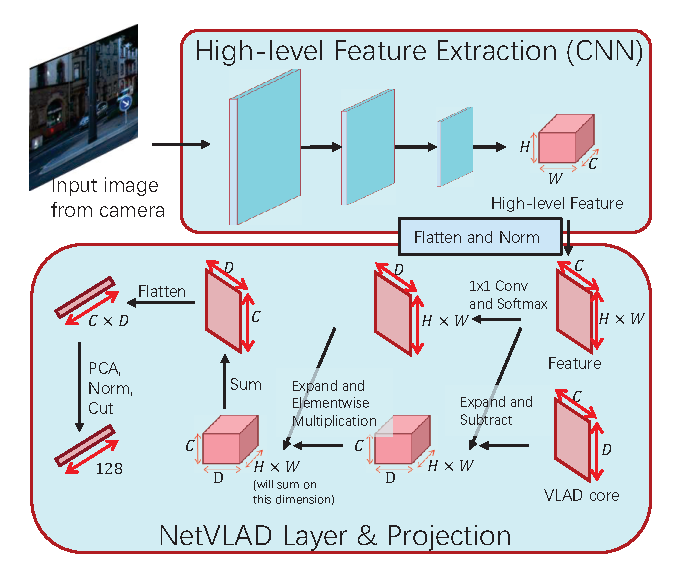
\includegraphics[width=0.85\linewidth]{fig/NetVLAD.eps}\label{fig:NetVLAD}} 
    \caption{Process of NetVLAD.}
\end{figure}
